\chapter{Proposed Approach and Methodology}
\label{ch:method}

This chapter describes how we will build and evaluate the diagnostic core of KhetLens: the data, the model and its training, its compression for the phone, the weather-aware adjustment, the uncertainty check with follow-up questions, the field-data study, and the evaluation plan. We describe the algorithms and procedures rather than code. Figure~\ref{fig:pipeline} shows the overall pipeline.

\begin{figure}[H]
  \centering
  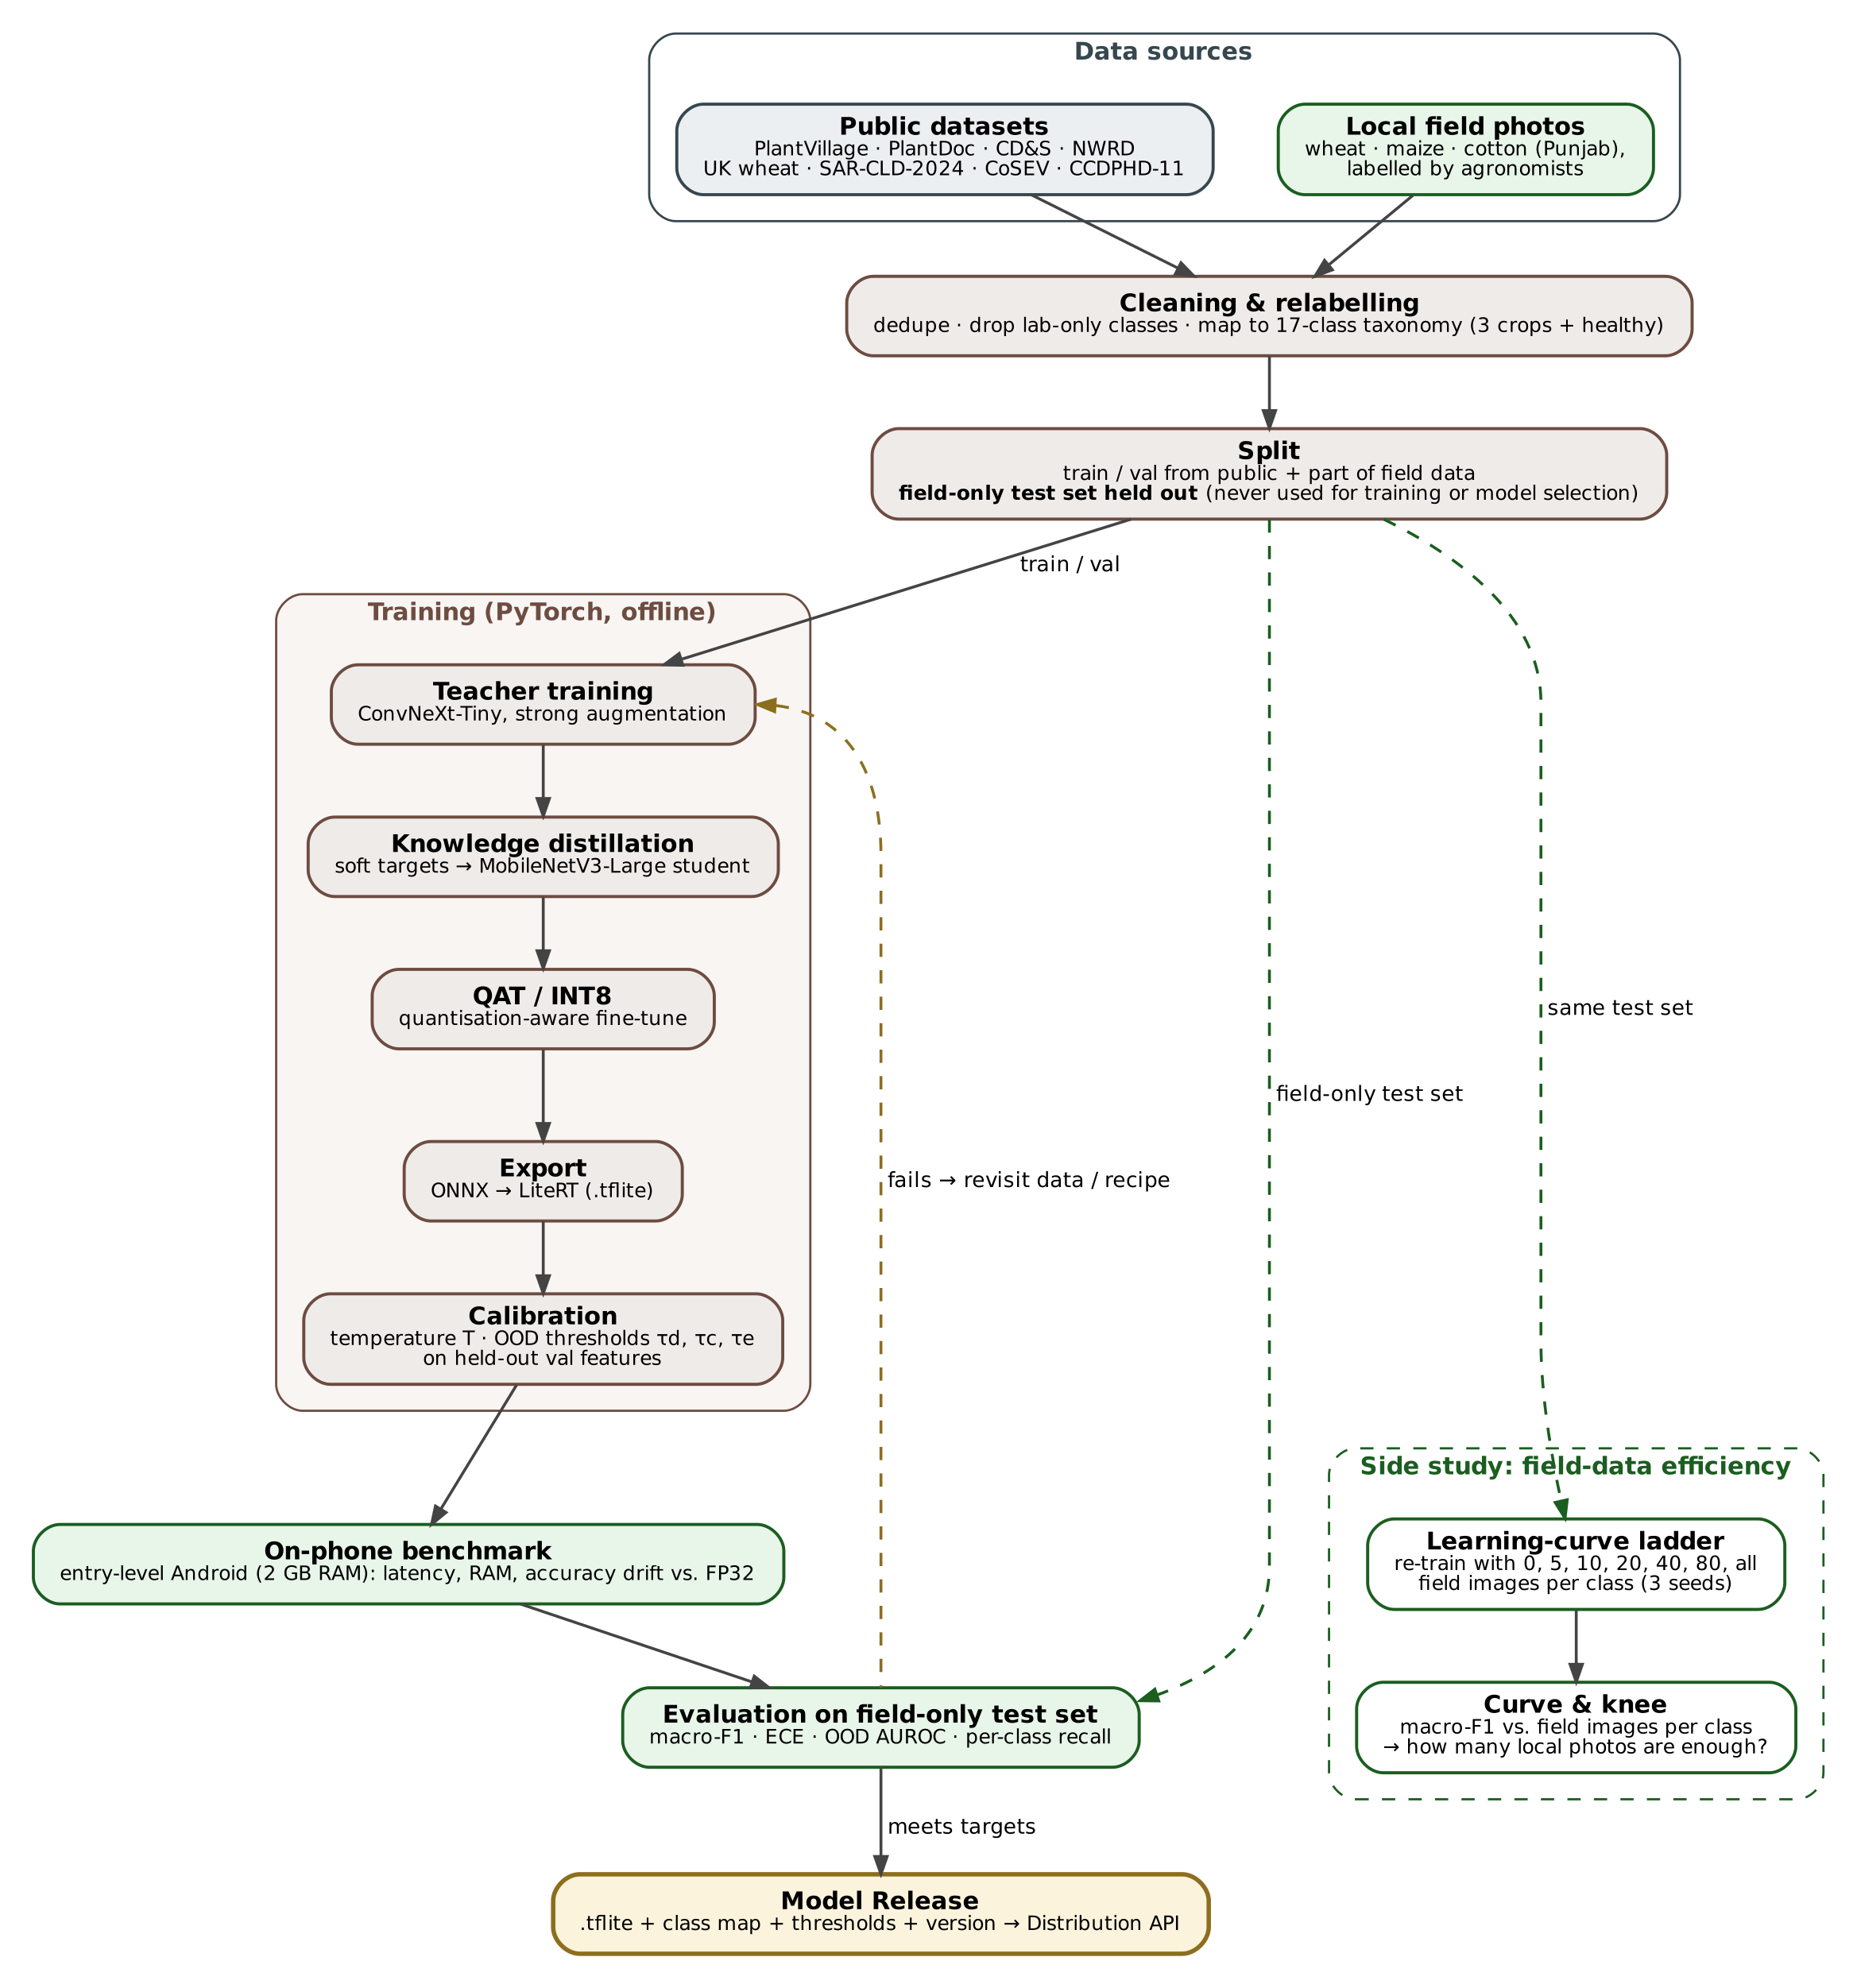
\includegraphics[width=\textwidth,height=0.88\textheight,keepaspectratio]{Figures/diagrams/pipeline_methodology.png}
  \caption{Training and deployment pipeline. Public datasets and local field photographs are mapped to the 17-class taxonomy; a field-only test set is held out; a larger teacher is trained and distilled into a MobileNetV3 student, which is quantised, exported, calibrated, benchmarked on entry-level phones and released. The field-data study branches from the same data.}
  \label{fig:pipeline}
\end{figure}

\section{Overview of the Approach}
Five principles, each drawn from the literature in Chapter~\ref{ch:lit}, guide the approach. We evaluate on field photographs, because that is where the application will be used. We train a large model and deploy a small one, using distillation and quantisation to keep most of the accuracy. We bring weather into the diagnosis as reviewed knowledge rather than as a learned input, because that needs no paired data and can be checked by agronomists. We check every input before answering, so that the app asks or declines rather than guesses. And we treat the amount of local data needed as a question to be measured rather than assumed.

\section{Data Strategy}
\label{sec:data}
\subsection{Taxonomy and sources}
All sources are mapped to the 17-class taxonomy of Table~\ref{tab:classes}; each source class maps to one KhetLens class or is left out, and the mapping is kept in a configuration file so the dataset can be rebuilt. Table~\ref{tab:datasets} lists the public sources we have identified. They come from several regions, which is a strength: variety in background, lighting and camera helps the model generalise. Local field photographs collected with our partner complete the picture for Punjab's conditions.

\begin{table}[H]
\centering\small
\caption{Public image sources mapped to the taxonomy.}
\label{tab:datasets}
\begin{tabularx}{\textwidth}{|L{3.6cm}|L{1.4cm}|L{2.6cm}|Y|}
\hline
\textbf{Source} & \textbf{Crop} & \textbf{Setting} & \textbf{Classes used} \\ \hline
PlantVillage~\cite{hughes2015plantvillage} & Maize & Laboratory & NLB, common rust, GLS, healthy \\ \hline
PlantDoc~\cite{singh2020plantdoc} & Maize & Field & NLB, rust, GLS \\ \hline
CD\&S~\cite{ahmad2021cds} & Maize & Field & NLB, GLS \\ \hline
NWRD~\cite{anwar2023nwrd} & Wheat & Field, Pakistan & Yellow (stripe) rust \\ \hline
Wheat field set~\cite{long2024ukwheat} & Wheat & Field and glasshouse & Yellow rust, brown rust, powdery mildew, Septoria leaf blotch (mapped to leaf blight), healthy \\ \hline
Punjab/KP wheat~\cite{malik2025wheatpk} & Wheat & Field and lab, Pakistan & Yellow and brown rust, powdery mildew, healthy \\ \hline
SAR-CLD-2024~\cite{sarcld2024} & Cotton & Field & Bacterial blight, leaf curl, reddening, leaf-hopper damage, healthy (subset of its seven classes) \\ \hline
CoSEV~\cite{noon2023cosev} & Cotton & Field, Pakistan & Leaf curl virus \\ \hline
CCDPHD-11~\cite{wang2025cotton} & Cotton & Mixed (online and field) & Bacterial blight, leaf curl, reddening, target spot (fungal leaf spot), pest damage, healthy \\ \hline
Pakistani cotton set~\cite{anwarcotton2023pk} & Cotton & Field and web & Healthy, bacterial blight, leaf curl \\ \hline
PlantWild~\cite{wei2024plantwild} & Various & In the wild & Plant-domain pre-training; non-target crops for OOD tests \\ \hline
\end{tabularx}
\end{table}

\subsection{Local field collection}
We collect photographs with our partner's field officers during the wheat season (winter) and the maize and cotton season (summer), using the same class of phone farmers own, under the lighting and backgrounds found at the time of the visit, with several leaves per plant. Each photograph is tagged with crop, date, district and growth stage, and an agronomist assigns the label. A subset is labelled by a second agronomist so that we can measure agreement. Unlabelled photographs are kept for self-supervised pre-training, and photographs of non-target crops and non-leaf scenes are collected as out-of-distribution test material.

\subsection{Splits and pre-processing}
We keep three disjoint sets. The training pool contains the public data plus the local photographs released to training. A validation set, stratified from the pool, is used for early stopping, temperature fitting and threshold selection. The field test set contains only local field photographs, split by plant so that no leaf of the same plant appears in both training and test, and is never used for tuning. Images are resized to 224 pixels for training with random crops at a range of scales, flips, colour jitter bounded to preserve lesion colour, and photometric distortions that imitate phone cameras (re-compression, mild blur, exposure shifts). To reduce background shortcuts, laboratory images are also composited onto field backgrounds. Class imbalance is handled by balanced sampling.

\section{Model Architecture}
\label{sec:model}
The deployed model is one network with a shared backbone and several heads, following the crop-conditional design that improved field accuracy in Picon et al.~\cite{picon2019cropcond}:
\begin{itemize}
  \item \textbf{Backbone:} MobileNetV3-Large~\cite{howard2019mnv3}, pre-trained on ImageNet and, where it helps, further pre-trained on plant images. It produces a feature vector $f(x)$ for the image.
  \item \textbf{Crop head:} three outputs (wheat, maize, cotton).
  \item \textbf{Disease heads:} one per crop with 6, 5 and 6 outputs; at inference only the head of the detected (or farmer-confirmed) crop is read.
\end{itemize}
The heads are trained together, each disease head receiving gradient only from images of its crop. We use an additive-margin softmax loss rather than plain cross-entropy, because margin losses make class clusters tighter and help the unknown-disease check~\cite{meng2023osr}. MobileNetV3-Small, EfficientNet-Lite and a MobileViT-class hybrid~\cite{tonmoy2025mobileplantvit} are trained with the same heads as benchmarked alternatives.

\subsection{Close-up and wider photographs}
\label{sec:multiscale}
Farmers will not always photograph a single leaf; many will photograph the affected plant from a short distance, with several leaves and part of the crop in view. We handle both kinds of photograph with the same model in two ways. During training, the images from field datasets already include a range of distances, and we add scale augmentation (random crops covering from a small part to the whole image) so that the model sees symptoms at different sizes. At inference, the photograph is classified as a whole and also as a small grid of overlapping regions; each region's probabilities are weighted by how confident the model is about it and averaged with the whole-image result. For a close-up this reduces to the ordinary single prediction; for a wider shot it lets the regions that contain affected leaves carry the decision. This adds only a few extra passes of the compact model and keeps the response time within our target.

\section{Training by Knowledge Distillation}
\label{sec:kd}
We first train a larger \emph{teacher} (ConvNeXt-Tiny, with the same head structure) on the training pool. The \emph{student} is then trained to match both the labels and the teacher's softened outputs~\cite{hinton2015kd}:
\begin{equation}
\mathcal{L}_{\text{KD}} = (1-\alpha)\,\mathcal{L}\big(y, \sigma(z_s)\big) + \alpha\, T_{\text{KD}}^2\, \mathrm{KL}\!\left( \sigma\!\left(\tfrac{z_t}{T_{\text{KD}}}\right) \,\middle\|\, \sigma\!\left(\tfrac{z_s}{T_{\text{KD}}}\right) \right),
\label{eq:kd}
\end{equation}
where $z_t$ and $z_s$ are the teacher's and student's logits, $\sigma$ is the softmax, $T_{\text{KD}}$ is the distillation temperature and $\alpha$ weights the two terms; both are chosen on the validation set. The value $\mathcal{L}_{\text{KD}}$ is the training loss we minimise: its first term measures how far the student's prediction is from the true label, its second how far the student's softened output is from the teacher's, so a low value means the student both predicts correctly and reproduces the teacher's view of which classes resemble each other. We run each reported configuration with three random seeds and report the mean and spread.

\section{Compression and Deployment}
\label{sec:deploy}
After training, the student is fine-tuned briefly with quantisation-aware training so that weights and activations can be stored as 8-bit integers with little loss~\cite{krishnamoorthi2018quant}. The calibration data include field images in proportion. We record accuracy before and after quantisation, and a release is held back if the drop on the field test set is more than a small margin. The model is exported to ONNX and converted to a TensorFlow Lite flatbuffer with full integer quantisation; the same graph is also packaged for ONNX Runtime so that the two runtimes can be compared on the phone~\cite{zhangq2022mobilebench}. The release bundle contains the model, the class map, the input size, the calibration temperature, the statistics used by the novelty check, and the thresholds.

\textbf{On-device benchmark.} On entry-level Android phones, after a short warm-up, we time a few hundred inferences and record the median and 95th-percentile latency, start-up time, peak memory and battery use for each runtime and input size. These measurements guide the final choice of runtime and input size.

\section{Context-Aware Fusion}
\label{sec:fusion}
Figure~\ref{fig:fusion} illustrates the weather adjustment. Let $p(y \mid x)$ be the calibrated probability of each condition $y$ of the detected crop for image $x$, and let $w$ summarise the district's weather over the preceding two weeks: mean daily maximum and minimum temperature, mean relative humidity, total rainfall and days since rain. A \emph{plausibility prior} $\pi(y \mid w)$, between a floor $\pi_{\min}$ and 1, is read from a lookup table built from epidemiological literature and reviewed by agronomists. The adjusted result is
\begin{equation}
\tilde{p}(y \mid x, w) = \frac{p(y \mid x)\, \pi(y \mid w)^{\lambda}}{\sum_{y'} p(y' \mid x)\, \pi(y' \mid w)^{\lambda}},
\label{eq:fusion}
\end{equation}
where $\lambda \in [0,1]$ sets how strongly the weather is allowed to influence the result. The value $\tilde{p}(y \mid x, w)$ is the adjusted probability of each condition given both the photograph and the recent weather; the conditions still sum to one, and the condition with the highest $\tilde{p}$ is the one shown to the farmer. The floor $\pi_{\min}$ means the weather can make a condition less likely but never rule it out, and when no recent weather is stored the prior is uniform and the result screen says so.

\begin{figure}[H]
  \centering
  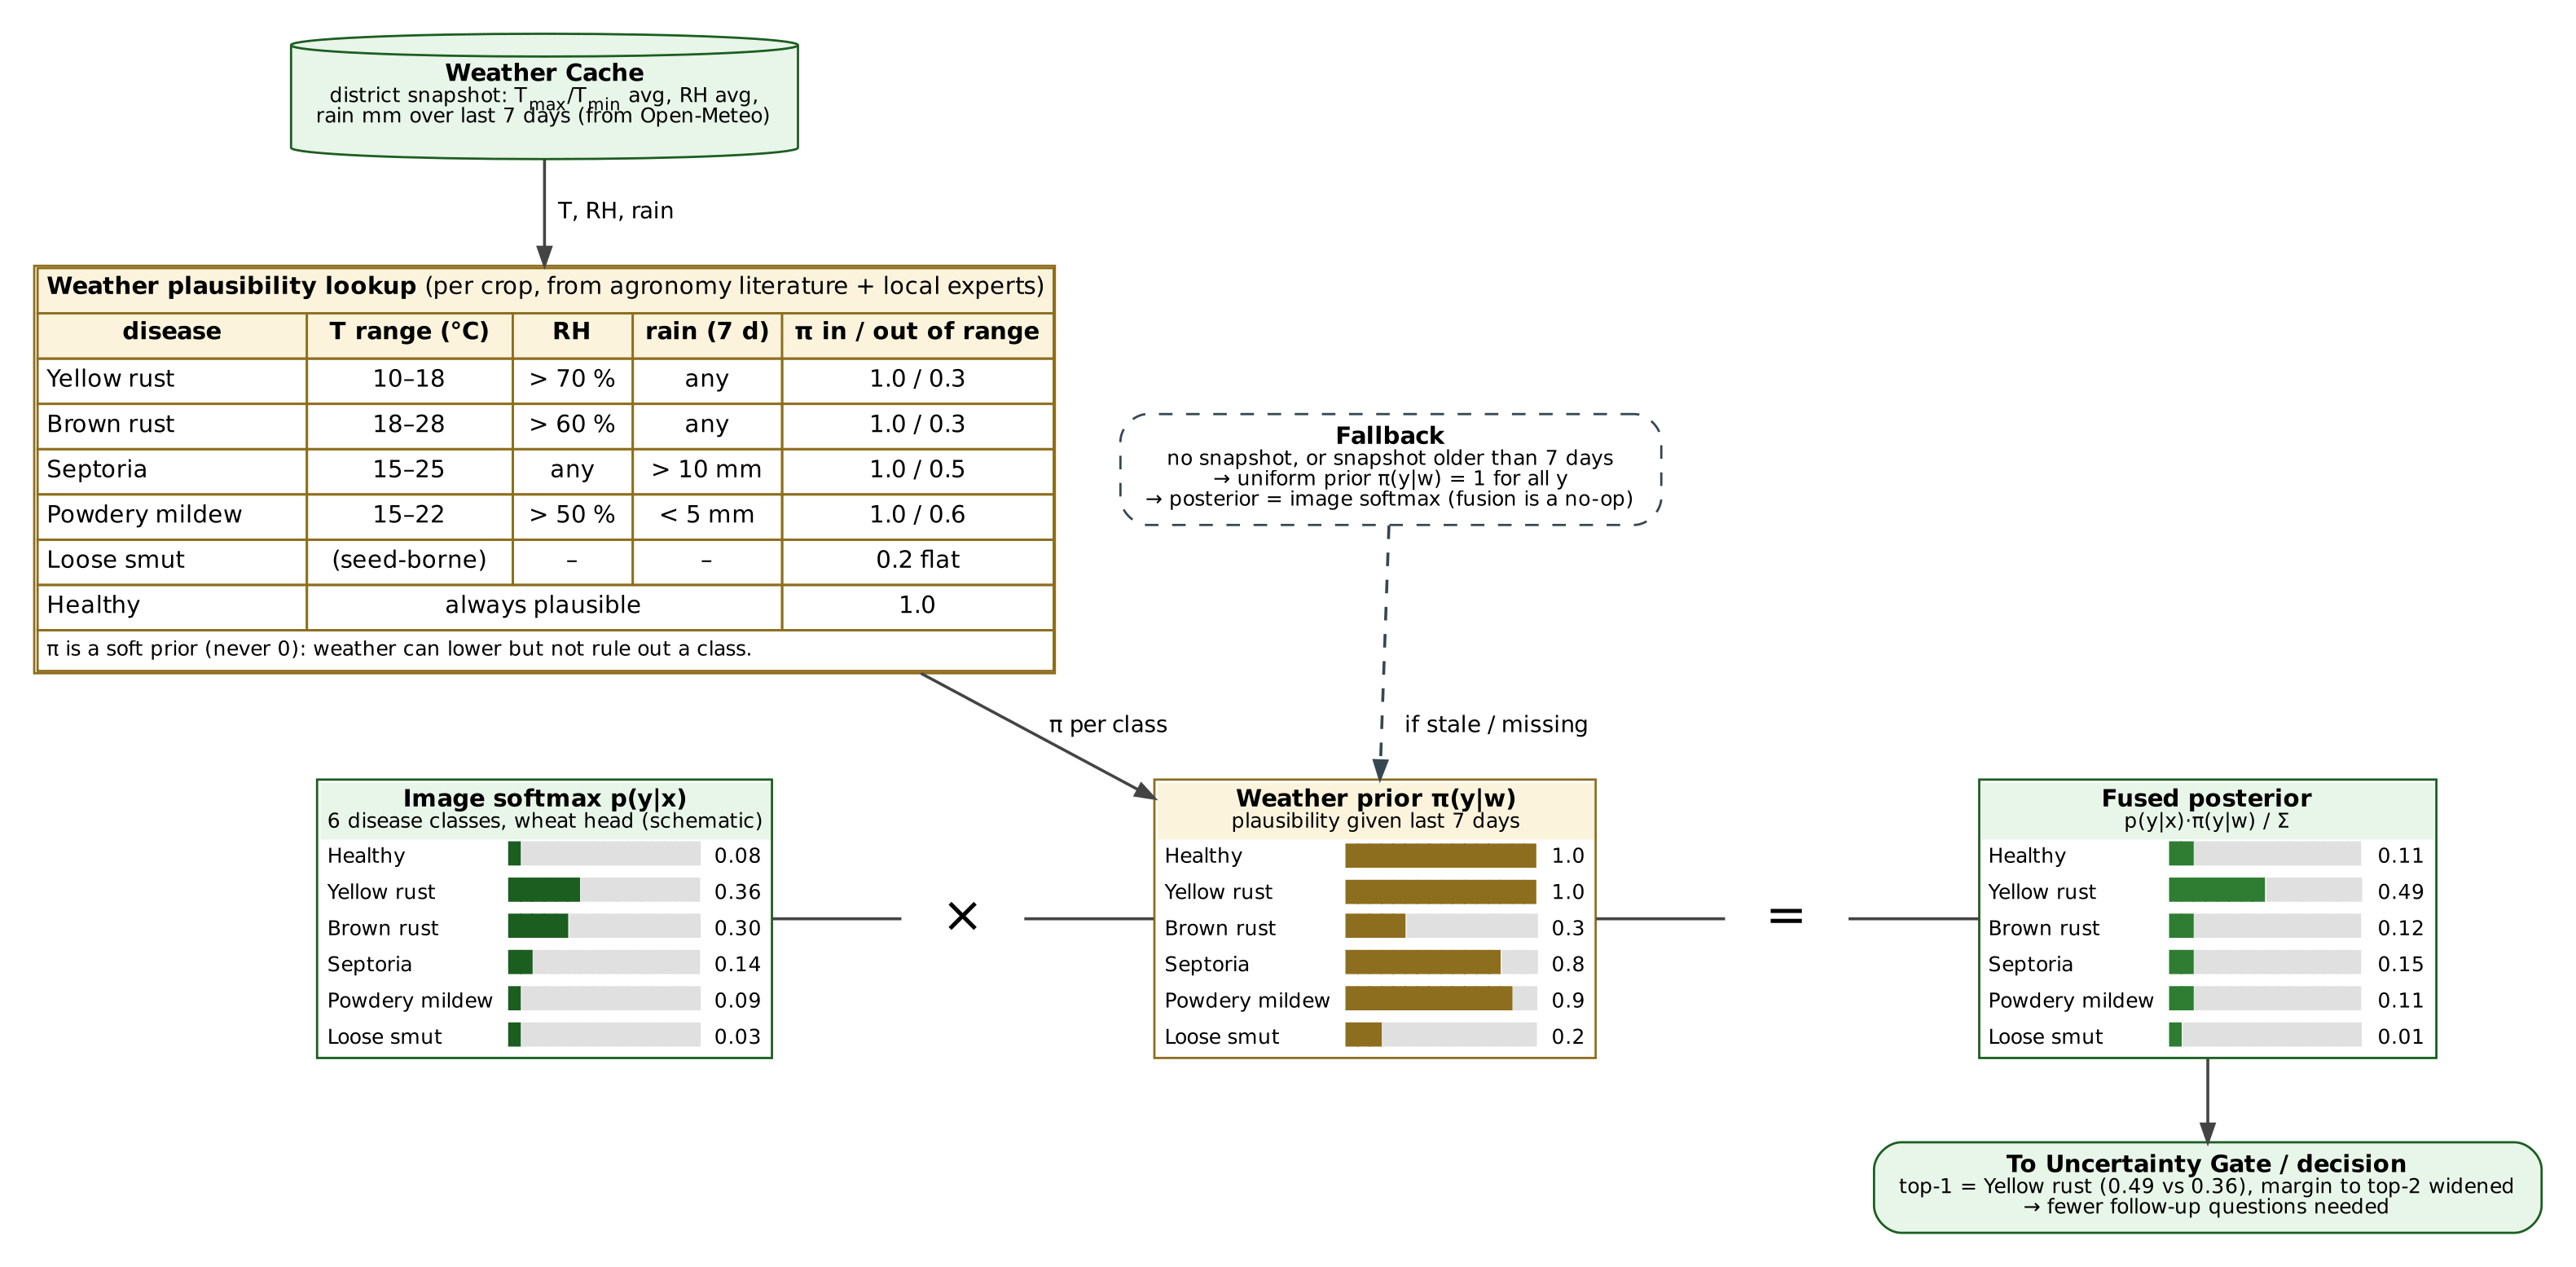
\includegraphics[width=\textwidth,height=0.88\textheight,keepaspectratio]{Figures/diagrams/fusion_diagram.png}
  \caption{Weather-aware adjustment (shown with $\lambda = 1$). The classifier's probabilities over the crop's conditions are multiplied by a plausibility prior read from a lookup table and renormalised. Bars are illustrative. When no recent weather is stored, the prior is uniform.}
  \label{fig:fusion}
\end{figure}

Table~\ref{tab:prior} gives an illustrative excerpt of the table for wheat. The stripe rust row uses the ranges fitted on Punjab data by Ali et al.~\cite{ali2023striperust}; the other rows are our initial proposals and will be set with the agronomists. The table is part of the content pack, so it can be refined without changing the model. The value of $\lambda$ is chosen on the validation set by looking at the designated look-alike pairs (Section~\ref{sec:pairs}), with the condition that no class loses accuracy, and the result with $\lambda = 0$ is always reported alongside.

\begin{table}[H]
\centering\small
\caption{Illustrative weather plausibility table for wheat (excerpt, to be set with agronomists).}
\label{tab:prior}
\begin{tabularx}{\textwidth}{|L{2.8cm}|Y|L{1.2cm}|}
\hline
\textbf{Condition} & \textbf{Rule on the two-week summary} & \textbf{$\pi$} \\ \hline
Yellow rust & Daily maxima mostly 13--23\,$^\circ$C and humidity 50--85\%~\cite{ali2023striperust} & 1.0 \\
 & One of the two holds & 0.7 \\
 & Neither holds (for example, hot and dry) & 0.3 \\ \hline
Powdery mildew & Humid with little rain & 1.0 \\
 & Otherwise & 0.6 \\ \hline
Leaf blight & Recent rain and warm & 1.0 \\
 & Otherwise & 0.6 \\ \hline
Abiotic stress & Hot spell or long dry period & 1.0 \\
 & Otherwise & 0.5 \\ \hline
Healthy & Always & 1.0 \\ \hline
\end{tabularx}
\end{table}

\section{Uncertainty Check and Follow-Up Questions}
\label{sec:gate}
Figure~\ref{fig:gate} shows the uncertainty check as a flowchart and Algorithm~\ref{algo:gate} gives the procedure. Three signals are computed from the model's outputs; for a wider photograph, the feature vector and logits used below are the combined whole-image and region results of Section~\ref{sec:multiscale}.

\begin{figure}[H]
  \centering
  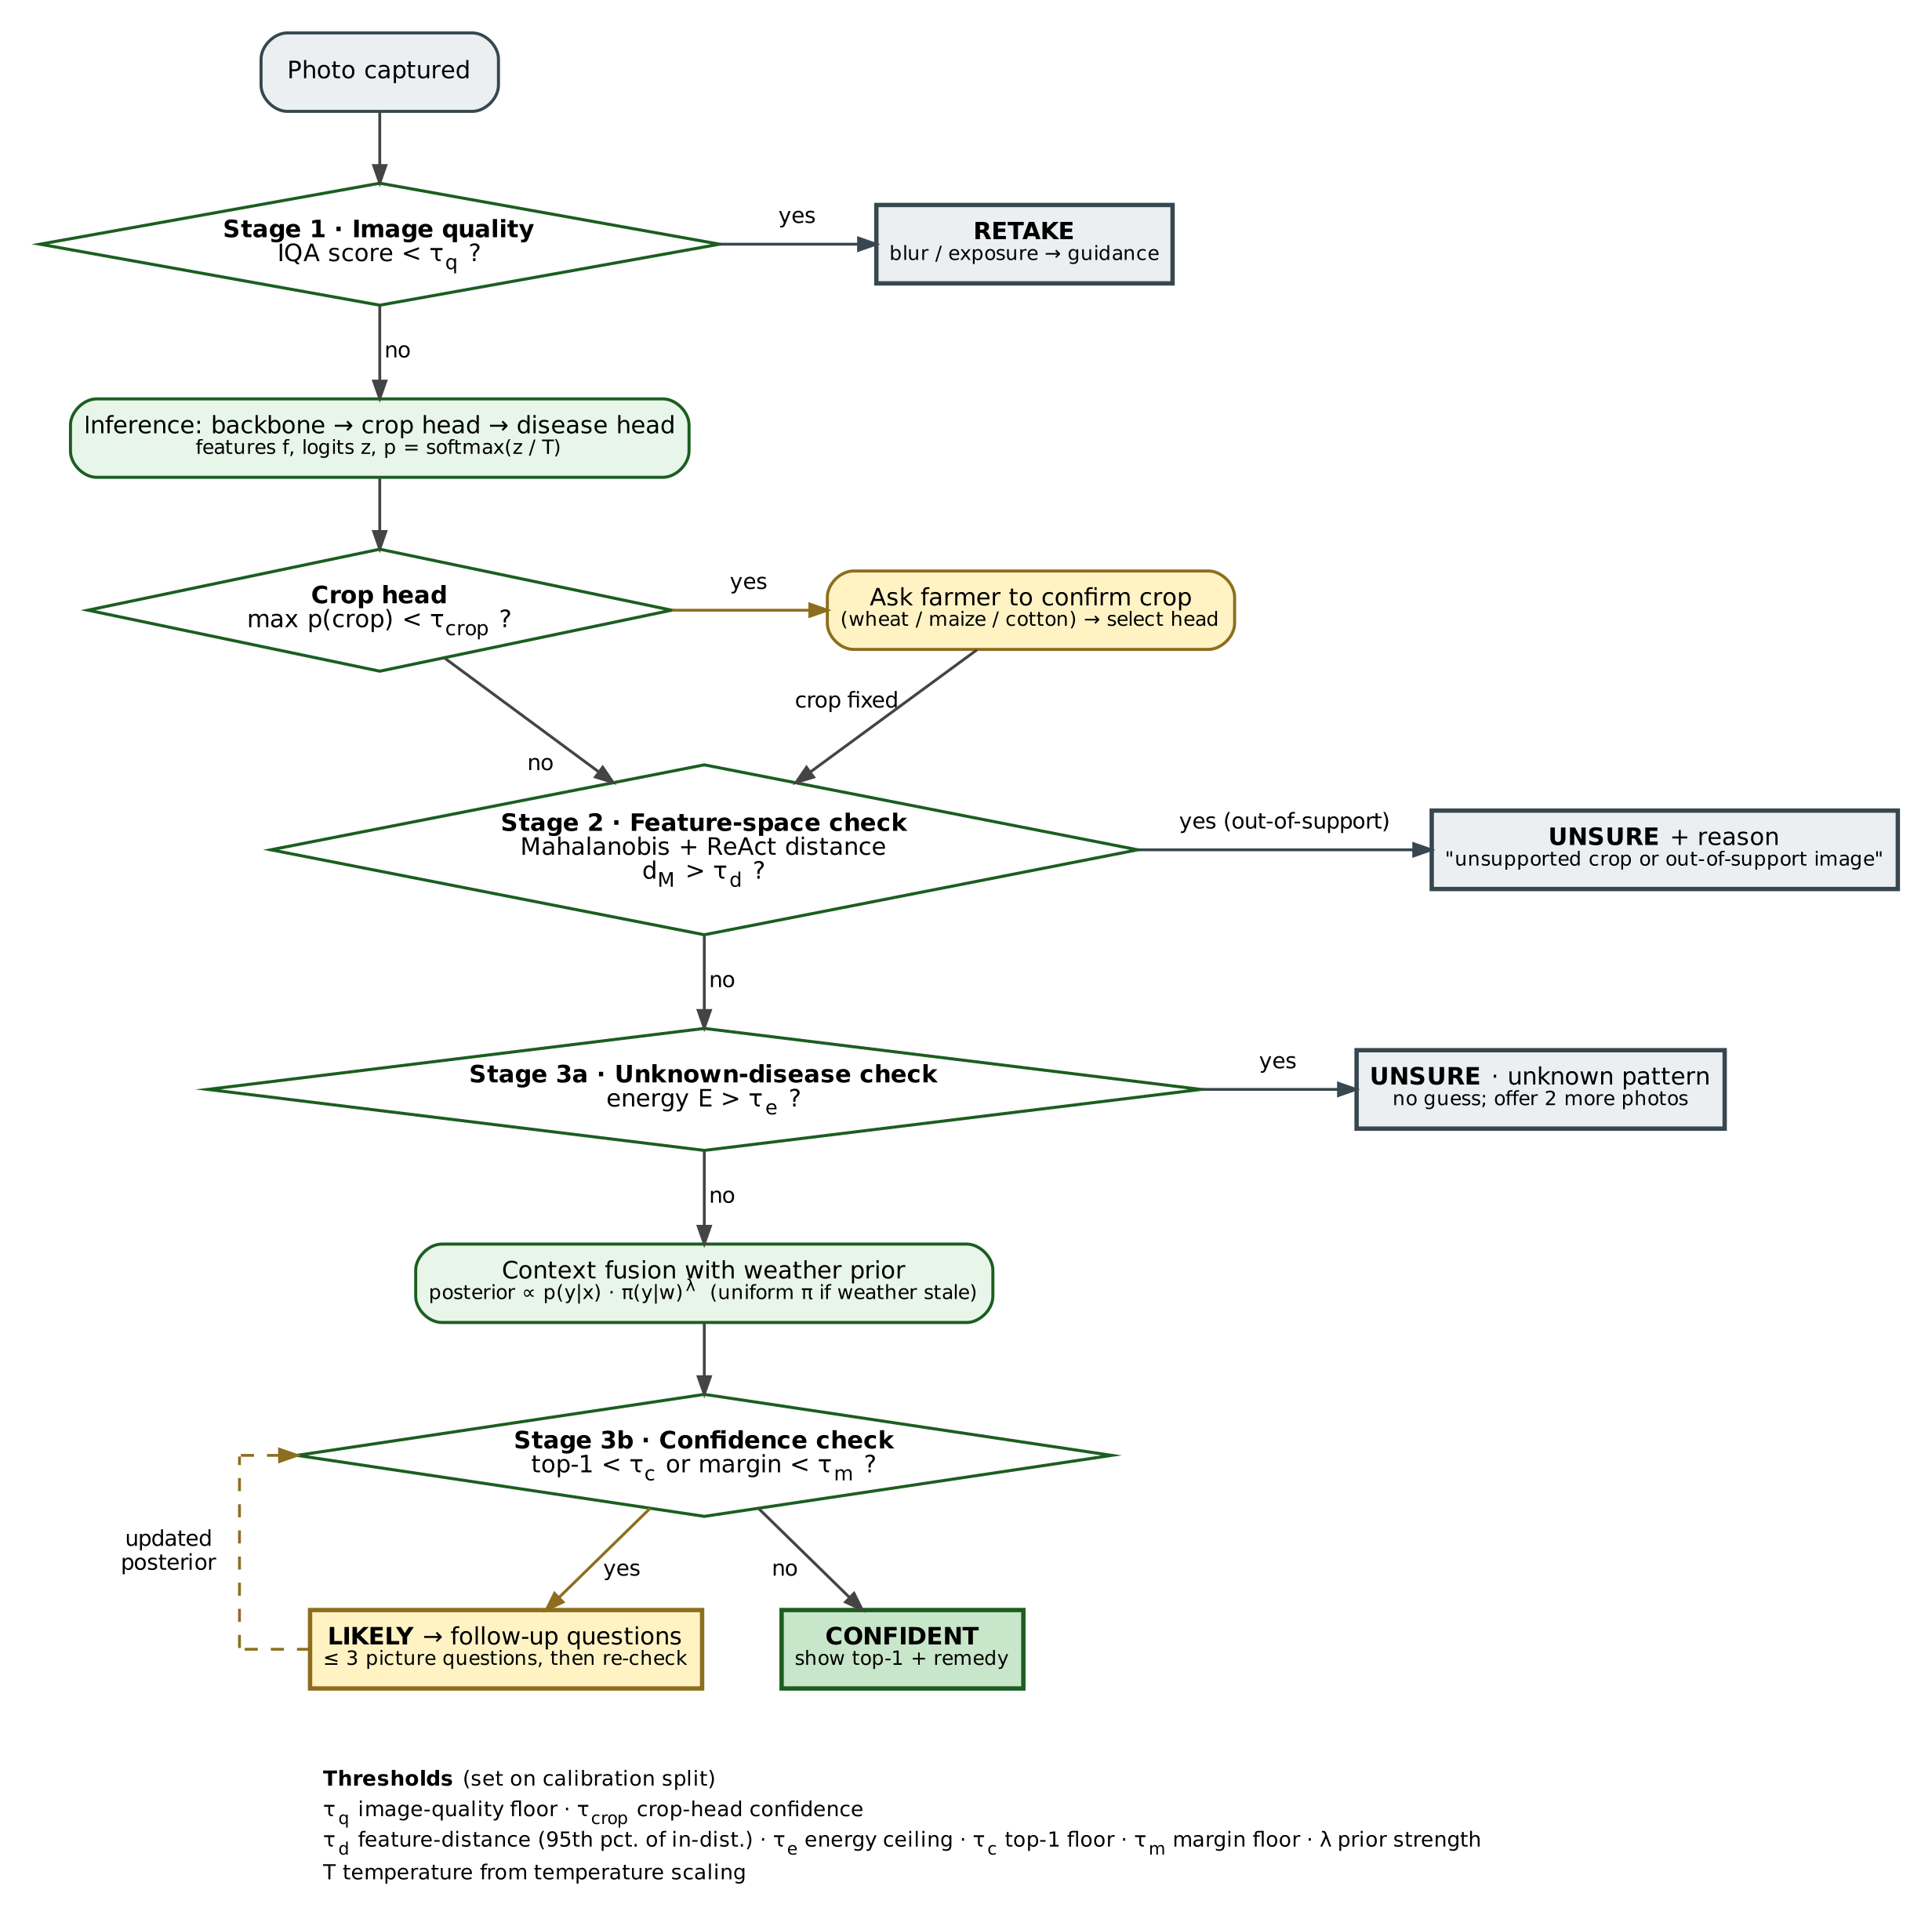
\includegraphics[width=\textwidth,height=0.88\textheight,keepaspectratio]{Figures/diagrams/gate_flowchart.png}
  \caption{The three-stage uncertainty check. Stage~1 rejects unusable photographs; Stage~2 recognises unsupported crops and other out-of-support images by feature distance; Stage~3a declines unfamiliar patterns by energy score before the weather adjustment, and Stage~3b sends low-confidence or near-tie results to follow-up questions after it. Thresholds are set on field data and shipped with the model.}
  \label{fig:gate}
\end{figure}

\textbf{Stage 1: image quality.} Before inference, a sharpness measure (variance of the Laplacian of the grey image) and an exposure measure (fraction of very dark or very bright pixels) are combined into a quality score, following the idea of a quality gate in AgroPath~\cite{ahmed2022agropath}. Below a threshold $\tau_q$ the photograph is sent back for a retake with the reason.

\textbf{Stage 2: feature-space novelty.} The backbone features are first clipped as in ReAct~\cite{sun2021react}, $f'(x) = \min(f(x), \kappa)$, and the Mahalanobis distance to the nearest class of the detected crop is then computed~\cite{lee2018mahalanobis}; combining the two is our own choice, and we will also evaluate the distance without clipping:
\begin{equation}
d_M(x) = \min_{k} \big(f'(x) - \mu_k\big)^{\!\top} \Sigma^{-1} \big(f'(x) - \mu_k\big),
\label{eq:maha}
\end{equation}
with class means $\mu_k$ and a shared covariance $\Sigma$ estimated on the training set and stored with the model. The value $d_M(x)$ measures how far the photograph's features lie from the nearest known class, scaled by how spread out that class normally is; a small value means the photograph looks like something the model was trained on, a large value means it does not. If $d_M(x)$ exceeds $\tau_d$ the input is treated as unsupported. Before this check, a crop-head confidence below $\tau_{crop}$ triggers a crop-confirmation prompt instead.

\textbf{Stage 3a: unknown-disease check.} The energy score $E(x) = -T \log \sum_k \exp(z_k / T)$~\cite{liu2020energy}, where $z_k$ are the logits of the crop's disease head and $T$ the calibration temperature, summarises how strongly the model responds to the image overall: a low (more negative) value means at least one class fired strongly, a high value means no class did, which is typical of an unfamiliar pattern. It is compared with the softmax baseline~\cite{hendrycks2017msp} during evaluation, and the better of the two on held-out diseases is shipped. Above its threshold $\tau_e$ the outcome is Unsure with reason ``unfamiliar pattern'', and the farmer is offered two more photographs. In Algorithm~\ref{algo:gate} this score is written as $E$; if the softmax score wins the comparison it takes the same place.

\textbf{Stage 3b: calibrated confidence.} Logits are temperature-scaled~\cite{guo2017calibration}, $p = \sigma(z/T)$, with $T$ fitted on the validation set; the resulting $p$ is a probability for each condition whose value matches how often the model is actually right at that level, so that ``87\%'' on the result screen means roughly 87 in 100 such results are correct. After the weather adjustment, if the top probability is at least $\tau_c$ and the margin over the second is at least $\tau_m$, the outcome is Confident; otherwise it is Likely and the follow-up questions begin.

Thresholds are set on the validation set: $\tau_q$ to send most blurred photographs for retake while rarely rejecting sharp ones; $\tau_{crop}$ to ask for crop confirmation only when the crop head is genuinely unsure; $\tau_d$ and $\tau_e$ to keep nearly all supported inputs while rejecting as many out-of-support inputs as possible, tested against non-leaf images, leaves of other crops and held-out diseases; $\tau_c$ and $\tau_m$ to keep accuracy high on the results marked Confident. All thresholds ship in the model release and are re-fitted for each release.

\begin{algorithm}[H]
\small
\KwData{image $x$; weather summary $w$ (may be absent); model; release parameters $T, \mu, \Sigma^{-1}, \kappa, \tau_q, \tau_{crop}, \tau_d, \tau_e, \tau_c, \tau_m, \lambda$}
\KwResult{one of \textsc{Retake}, \textsc{ConfirmCrop}, \textsc{Confident}, \textsc{Likely}, \textsc{Unsure}}
$q \leftarrow \textsc{QualityScore}(x)$\;
\If{$q < \tau_q$}{\Return \textsc{Retake}(reason)\;}
$f \leftarrow \textsc{Backbone}(x)$; \quad $p_{crop} \leftarrow \sigma(\textsc{CropHead}(f))$\;
\If{$\max p_{crop} < \tau_{crop}$}{\Return \textsc{ConfirmCrop}($p_{crop}$)\;}
$c \leftarrow \arg\max p_{crop}$; \quad $z \leftarrow \textsc{DiseaseHead}_{c}(f)$\;
$d_M \leftarrow$ Equation~\ref{eq:maha} on $\min(f, \kappa)$\;
\If{$d_M > \tau_d$}{\Return \textsc{Unsure}(``unsupported'')\;}
$p \leftarrow \sigma(z / T)$; \quad $E \leftarrow -T\log\sum_k \exp(z_k/T)$\;
\If{$E > \tau_e$}{\Return \textsc{Unsure}(``unfamiliar pattern'')\;}
$\pi \leftarrow$ recent $w$ available ? \textsc{PriorTable}$(c, w)$ : uniform\;
$\tilde{p} \leftarrow p \odot \pi^{\lambda} / \sum (p \odot \pi^{\lambda})$\;
\eIf{$\tilde{p}_{(1)} \geq \tau_c \ \wedge\ \tilde{p}_{(1)} - \tilde{p}_{(2)} \geq \tau_m$}{
  \Return \textsc{Confident}($\arg\max \tilde{p}$, $\tilde{p}_{(1)}$, reasons)\;
}{
  \Return \textsc{Likely}(top two of $\tilde{p}$)\;
}
\caption{Diagnosis with the uncertainty check and weather adjustment.}
\label{algo:gate}
\end{algorithm}

\textbf{Follow-up questions.} For a Likely outcome, the app loads the crop's question set from the content pack. Each question has two or three illustrated options, and for each option and condition the pack stores a likelihood set by the agronomists on a coarse scale (typical, neutral, unlikely). After each answer the probabilities are updated by Bayes' rule, and ``Not sure'' leaves them unchanged. The next question is the one that best separates the remaining candidates, and the dialogue stops as soon as one condition dominates or after three questions, when the outcome becomes Unsure. This follows the conversational approach of DSSApple~\cite{sottocornola2022dssapple}. The ``take two more photos'' step averages the adjusted probabilities of all photographs that pass the first two stages and re-applies the third, following the multi-leaf finding of the Nuru field study~\cite{mrisho2020nuru}.

\section{Field-Data Efficiency Study}
\label{sec:study}
This study answers RQ2 with a learning-curve experiment; Figure~\ref{fig:study} shows the expected shape.

\begin{figure}[H]
  \centering
  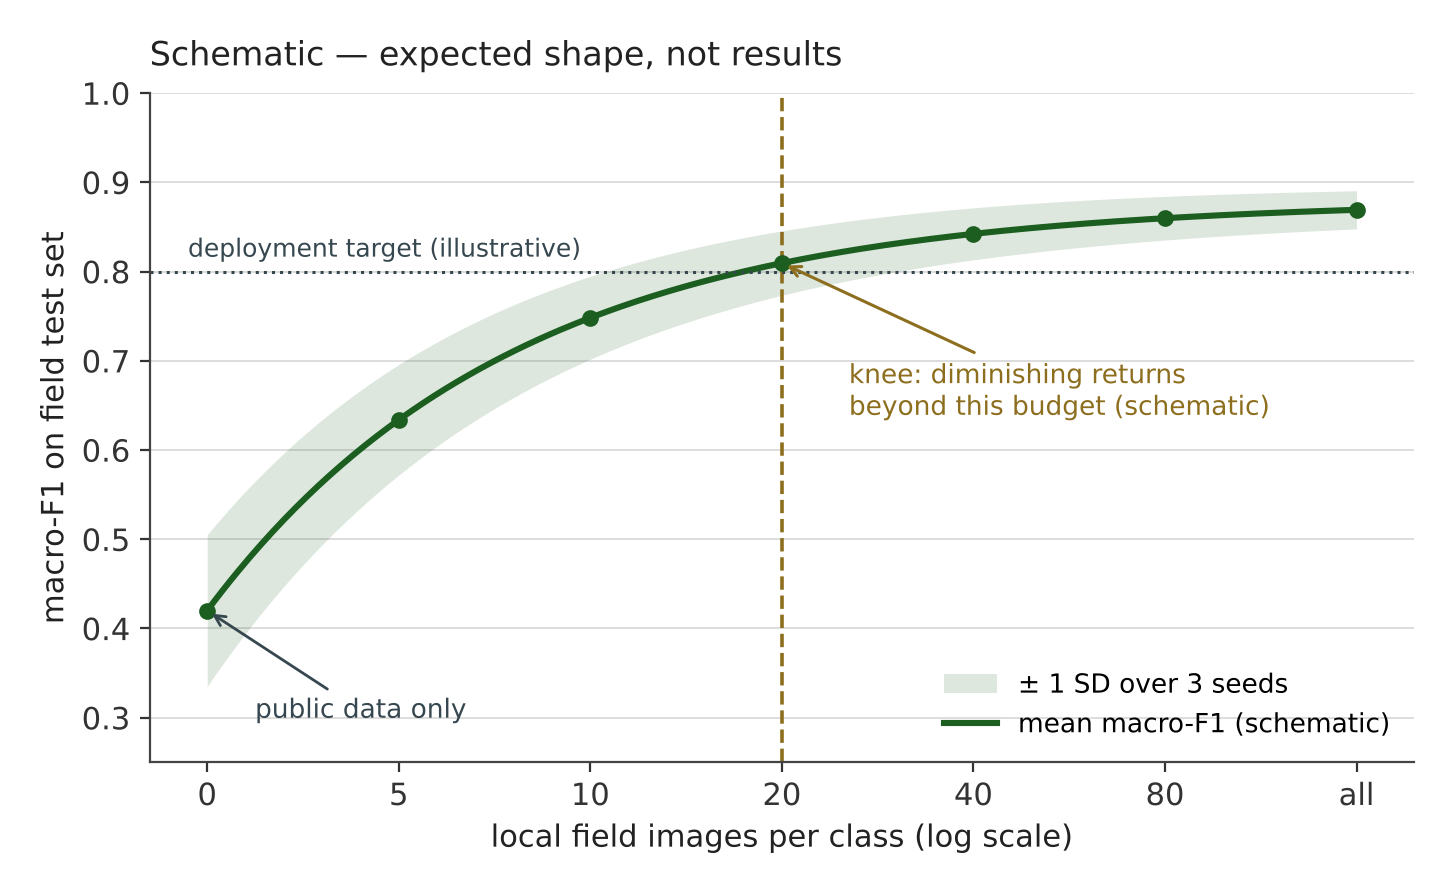
\includegraphics[width=\textwidth,height=0.88\textheight,keepaspectratio]{Figures/diagrams/study_design.png}
  \caption{Design of the field-data efficiency study (expected shape, not results). Macro-F1 on the fixed field test set is plotted against the number of local field images per class released to training; the band shows the spread across seeds and the knee marks diminishing returns.}
  \label{fig:study}
\end{figure}

The field test set is fixed first and never touched. For each point on a logarithmic ladder of local images per class (0, 5, 10, 20, 40, 80, and all available), and for each of three random seeds, a random subset of that size is added to the public training pool and the student is fine-tuned from the public-only checkpoint. The ladder matches the few-shot grids in the literature~\cite{argueso2020fewshot,xu2022transfer} so that our results can be compared with them. We report macro-F1 and per-class F1 on the field test set as mean and spread over seeds, per crop and overall, fit the power law $\text{err}(N) = a\,N^{\gamma} + \varepsilon_\infty$~\cite{beck2022curves}, where $\text{err}(N)$ is the error on the field test set after adding $N$ local images per class, $\gamma$ (negative) is how quickly error falls as data grows, $\varepsilon_\infty$ is the error that remains however much data is added, and $a$ is a scale constant; and report the knee as the smallest $N$ beyond which doubling the local data gains less than one point. Two secondary comparisons are run alongside: with and without self-supervised pre-training on the unlabelled local photographs, and random against uncertainty-based selection of which images to label. Each fine-tuning run is short enough that the full ladder fits within our compute allocation.

\section{Evaluation Plan}
\label{sec:eval}
Table~\ref{tab:evalplan} maps the research questions and objectives to experiments and metrics. All classification metrics are computed on the field test set; accuracy on laboratory images is reported only to show the size of the gap.

\begin{table}[H]
\centering\small
\caption{Evaluation plan.}
\label{tab:evalplan}
\begin{tabularx}{\textwidth}{|L{1.4cm}|Y|L{3.6cm}|}
\hline
\textbf{Question} & \textbf{Experiment} & \textbf{Metrics} \\ \hline
RQ1 & Train on public data; test on laboratory split, held-out public field sets and the local field test set; with and without background augmentation; teacher vs student vs quantised student. & Accuracy, macro-F1, per-class F1 \\ \hline
RQ2 & Learning-curve ladder (Section~\ref{sec:study}). & Macro-F1 against $N$, fitted curve, knee \\ \hline
RQ3 & Weather adjustment on and off; confusion on the look-alike pairs; behaviour with missing weather. & Macro-F1 on pairs, per-class change \\ \hline
RQ4 & Softmax vs energy vs Mahalanobis on three OOD sets; calibration before and after temperature scaling; quality check on degraded images. & AUROC, false-positive rate at 95\% recall, calibration error, retake rate \\ \hline
O2 & On-device benchmark (Section~\ref{sec:deploy}). & Latency, start-up, memory, battery \\ \hline
O6 & Task-based test with farmers through our partner. & Task completion, time, feedback \\ \hline
\end{tabularx}
\end{table}

\textbf{Ethics.} Field photograph collection and farmer testing follow a protocol agreed with our supervisor and shared with our partner: oral consent in the participant's language, voluntary participation, no capture of faces, photographs stored only on team systems, and results reported in aggregate. Server-side records hold a hashed phone number and the district only.

\section{Conclusion}
This chapter has set out our approach in enough detail to be reproduced: the sources and their mapping to the taxonomy, the field-collection protocol, a shared-backbone multi-head MobileNetV3 student distilled from a larger teacher, quantisation-aware compression with a release check, an on-device benchmark, a reviewable weather adjustment with a floor and a fallback, a three-stage uncertainty check with follow-up questions, and a seeded learning-curve study. Each choice is tied to a finding in Chapter~\ref{ch:lit} and each research question to an experiment. The next chapter describes the software that carries this core to the farmer.
